\chapter{Parte II}

Nella seconda parte delle progetto abbiamo sviluppato una rete neurale che non si limita ad approssimare la formula \ref{eqn:formula} ma tiene conto anche delle diffenze percettive dell'occhio umano. L'equazione infatti è imprecisa per certe zone dello spazio L*a*b e pertanto l'output della rete neurale precedente va corretto. Per fare ciò è necessario passare dallo spazio di colore CIE L*a*b allo spazio di colore CIE L*C*h ed infine definire delle regole di inferenza per un sistema fuzzy di tipo Madamani.
Ricordiamo gli intervalli delle coordinate nello spazio L*C*h.
\begin{itemize}
	\item \textit{Lightness (L\textsuperscript{*})} Range [0, 100]
	\item \textit{Hue (h)} Range  [0, 360\textdegree] 
    \item \textit{Chroma (C\textsuperscript{*})} Il range dipende dal valore L\textsuperscript{*}. \(C\textsubscript{max}= 127\) quando 
    \(L\textsuperscript{*}=50\) cioè quando si è al centro dell'ellissoide descritto dall spazio L*C*h mentre è \(C\textsuperscript{*}=0\) quando \(L\textsuperscript{*}=0\) oppure \(L\textsuperscript{*}=100\). La relazione tra \(L\textsuperscript{*}\) e \(C\textsuperscript{*}\) quindi si può descrivere come un ellisse.
    	\begin{equation}\label{eqn:ellipse}
       		\frac{C^2}{127^2} + \frac{(L-50)^2}{50^2} = 1
       	\end{equation}
    Quindi \({C^{'}}\textsubscript{max}\) si può calcolare come
    	\begin{equation}\label{eqn:c_primo_max}
    		{C^{'}}\textsubscript{max} = 127\sqrt{1 - \frac{(L-50)^2}{50^2}}
    	\end{equation}
    Pertanto definiamo 
         \begin{equation}\label{eqn:cperc}
       		c\% = 100\frac{C}{ {C^{'}}\textsubscript{max}}
       	\end{equation}
    Il range di c\% è [0, 100] ed è questo ultimo valore che useremo per le regole di inferenza.
\end{itemize}

\begin{figure}
	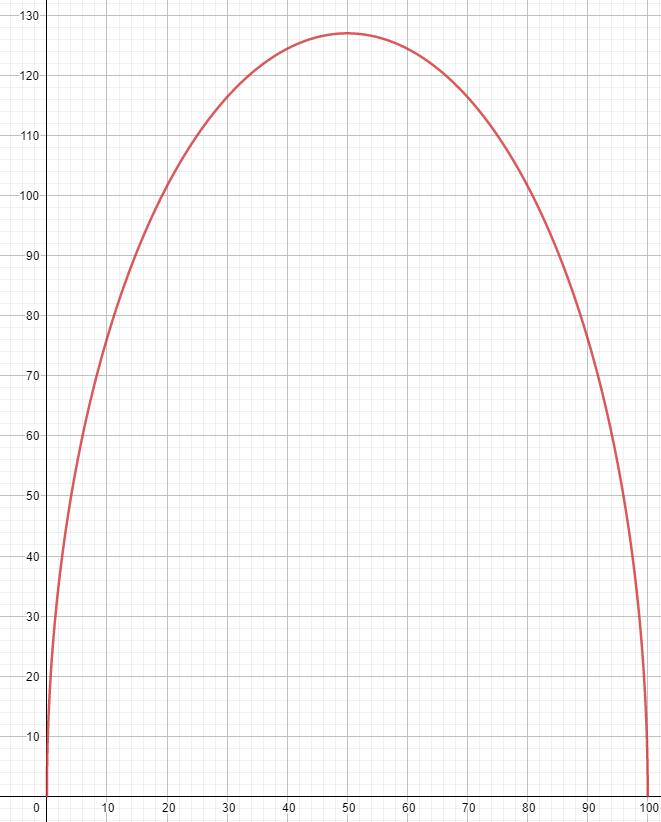
\includegraphics[scale=0.5]{images/geogebra-export.png}
\caption{Grafico del \({C^{'}}\textsubscript{max}\) al variare di L}
\end{figure}

\section{Membership function}